\documentclass{beamer}
\usepackage[latin1]{inputenc}
\usepackage{graphicx}
\usepackage{amsmath}
\usepackage{verbatim}
\usepackage{listings}
\usepackage{color}
\usetheme{Frankfurt}

\def\Tiny{\fontsize{4pt}{4pt}\selectfont}

\begin{document}

\usebackgroundtemplate
{
\includegraphics[height=\paperheight,width=\paperwidth]{pic/esrf_crisp/esrf_crisp_default.jpeg}
}

\begin{frame}{OHW2013 workshop}
\begin{center}
An open source PCIe device virtualization framework
\end{center}
\end{frame}

\setbeamertemplate{items}[circle]
\begin{frame}{Plan}
  \begin{itemize}
  \item Context and objectives
  \item Design and implementation
  \item Future directions
  \item Questions
  \end{itemize}
\end{frame}

%%
%% context

\begin{frame}{Context - ESRF and the ISDD electronic laboratory}
  \begin{center}
    \includegraphics[width=45mm]{pic/dv_esrf/main.jpg}
  \end{center}
  \begin{small}
    The ESRF is an XRAY light source for Europe located in Grenoble, France.
    The ISDD electronic laboratory mission is to develop and investigate
    \textbf{XRAY instrumentation electronics}.
  \end{small}
\end{frame}

\begin{frame}{Context - RASHPA}
  \begin{center}
    {
    \setlength{\fboxsep}{0pt}%
    \setlength{\fboxrule}{0pt}%
    \fbox{\includegraphics[width=50mm]{pic/dv_kc705/main.jpg}}
    \fbox{\includegraphics[width=50mm]{pic/dv_kc705_backend/main.jpeg}}
    }
  \end{center}
  \begin{tiny}
  \begin{itemize}
  \item high bandwidth data acquisition framework for 2D XRAY detectors
  \item Intel X86\_64 workstation
  \item KC705 prototype board, PCIe over cable
  \item see ICALEPCS poster session
  \end{itemize}
  \end{tiny}
\end{frame}

\begin{frame}{Context - DCORE}
  \begin{center}
    \includegraphics[width=50mm]{pic/dv_dcore/main.jpg}
  \end{center}
  \begin{small}
  \begin{itemize}
  \item generic data acquisition and control boards
  \item Intel ATOM CPU
  \item Xilinx Spartan6 FPGA
  \end{itemize}
  \end{small}
\end{frame}

\begin{frame}{Context - DUB}
  \begin{center}
    \includegraphics[width=50mm]{pic/dv_dub/main.jpg}
  \end{center}
  \begin{small}
  \begin{itemize}
  \item project specific readout electronics
  \item Intel ATOM CPU
  \item Xilinx Virtex6 FPGA
  \end{itemize}
  \end{small}
\end{frame}


%%
%% VPCIe

\begin{frame}{VPCIe - rationale}
  \begin{center}
    \includegraphics[width=65mm]{pic/dv_generic_platform/main.jpeg}
  \end{center}
  \begin{small}
  The above boards rely on \textbf{PCIe} as the default CPU to FPGA
  communication link. VPCIe is a framework made to \textbf{virtualize}
  these platforms on a standard desktop PC.
  \end{small}
\end{frame}

\begin{frame}{VPCIe - objectives}
  \begin{itemize}
  \item CPU software must run \textbf{unmodified} (including \textbf{drivers})
  \item few modifications allowed for \textbf{functional VHDL simulation}
  \item run \textbf{multiple PCIe devices} concurrently
  \item performances not critical
  \end{itemize}
\end{frame}

\begin{frame}{VPCIe - benefits}
  \begin{itemize}
  \item hardware software \textbf{codesign}
  \item \textbf{reduce} development cycle time
  \item platform \textbf{scaling} (multiple PCIe devices)
  \item test with \textbf{different CPU architectures} (INTEL, ARM ...)
  \item investigate \textbf{unavailable technologies} (NVM EXPRESS ...)
  \item \textbf{testing} (fault injection ...)
  \end{itemize}
\end{frame}

\begin{frame}{VPCIe - concepts}
  \begin{center}
    \includegraphics[width=50mm]{pic/dv_redirect/main.jpeg}
  \end{center}
  \begin{small}
    Applications on a \textbf{host} machine access hardware via interfaces. By
    \textbf{instrumenting} these interfaces, one can \textbf{redirect} the
    accesses to a software implementing the device. The device is said to be
    \textbf{virtualized}.
  \end{small}
\end{frame}

\begin{frame}{VPCIe - building blocks}
  VPCIe relies on opensource projects
  \newline

  \textbf{QEMU}
  \begin{itemize}
  \item http://wiki.qemu.org/Main\_Page
  \item architecture emulator (X86\_64, ARM ...)
  \item used to trap PCIe hardware accesses
  \end{itemize}

  \textbf{GHDL}
  \begin{itemize}
  \item http://ghdl.free.fr
  \item VHDL frontend for GCC
  \item used to implement device in VHDL
  \end{itemize}

\end{frame}

\begin{frame}{VPCIe - CPU virtualization}
  Full featured LINUX system
  \begin{itemize}
  \item runs in a QEMU virtual machine
  \item PCIe accesses are trapped and sent over TCP to the devices
  \item PCIe forwarder is available as a \textbf{QEMU patch}
    \setbeamertemplate{items}[triangle]
    \begin{itemize}
    \item maintainers contacted for a merge
    \end{itemize}
    \setbeamertemplate{items}[circle]
  \end{itemize}
\end{frame}

\begin{frame}{VPCIe - device virtualization}
  Virtual devices
  \begin{itemize}
  \item can be implemented in \textbf{C} or \textbf{VHDL}
    \setbeamertemplate{items}[triangle]
    \begin{itemize} 
    \item GHDL is used to compile VHDL into a \textbf{native executable}
    \item a glue interfaces the executable to the VPCIe runtime
    \end{itemize}
    \setbeamertemplate{items}[circle]
  \item run as a LINUX processes, can be \textbf{duplicated} at will
  \item PCIe made \textbf{simple}, focus on device logic
    \setbeamertemplate{items}[triangle]
    \begin{itemize}
    \item but close to the XILINX PCIe transaction layer
    \end{itemize}
    \setbeamertemplate{items}[circle]
  \end{itemize}
\end{frame}

\begin{frame}{VPCIe - implementation}
  \begin{center}
  \includegraphics[width=80mm]{pic/dv_implem/main.jpeg}
  \end{center}
\end{frame}

\begin{frame}{VPCIe - EBONE based example}
  \begin{center}
    \includegraphics[width=65mm]{pic/dv_generic_platform_vpcie/main.jpeg}
  \end{center}
  \begin{tiny}
    EBONE is a PCIe centric FPGA core interconnect developped at the ESRF
    and recently released on OHR (http://www.ohwr.org/projects/e-bone).\\
    Excluding the PCIe layer, most of the VHDL remains \textbf{unchanged}
    in a typical EBONE based design.
  \end{tiny}
\end{frame}

\begin{frame}[containsverbatim]
 \frametitle{VPCIe - virtualized device VHDL interface}
 \begin{tiny}
 \lstset{commentstyle=\color{blue}}
 \lstset{language=VHDL}
 \begin{lstlisting}[frame=tb]
entity endpoint is
 port
 (
  rst:          in std_ulogic;
  clk:          in std_ulogic;

  req_en:       out std_ulogic;
  req_wr:       out std_ulogic;
  req_bar:      out std_ulogic_vector(pcie.BAR_WIDTH - 1 downto 0);
  req_addr:     out std_ulogic_vector(pcie.ADDR_WIDTH - 1 downto 0);
  req_data:     out std_ulogic_vector(pcie.DATA_WIDTH - 1 downto 0);

  rep_en:       in std_ulogic;
  rep_data:     in std_ulogic_vector(pcie.DATA_WIDTH - 1 downto 0);

  mwr_en:       in std_ulogic;
  mwr_addr:     in std_ulogic_vector(pcie.ADDR_WIDTH - 1 downto 0);
  mwr_data:     in std_ulogic_vector(pcie.PAYLOAD_WIDTH - 1 downto 0);
  mwr_size:     in std_ulogic_vector(pcie.SIZE_WIDTH - 1 downto 0);

  msi_en:       in std_ulogic
 );
end entity;
 \end{lstlisting}
 \end{tiny}
\end{frame}

\begin{frame}[containsverbatim]
 \frametitle{VPCIe - virtualized device C interface}
 \begin{tiny}
 \lstset{commentstyle=\color{blue}}
 \lstset{language=C}
 \begin{lstlisting}[frame=tb]

/* runtime initialization */
int     pcie_init_net(pcie_dev_t*, ...);
int     pcie_fini(pcie_dev_t*);
int     pcie_loop(pcie_dev_t*);

/* misc config byte accessors */
int     pcie_set_deviceid(pcie_dev_t*, ...);
int     pcie_set_vendorid(pcie_dev_t*, ...);

/* PCIe BAR access handlers */
typedef void (*pcie_readfn_t)(uint64_t, void*, size_t, void*);
typedef void (*pcie_writefn_t)(uint64_t, const void*, size_t, void*);
int     pcie_set_bar(pcie_dev_t*, ..., pcie_readfn_t, pcie_writefn_t, ...);

/* host memory read write operations */
int     pcie_write_host_mem(pcie_dev_t*, uint64_t, size_t*);
int     pcie_read_host_mem(pcie_dev_t*, uint64_t, size_t*);

/* send an MSI */
int     pcie_send_msi(pcie_dev_t*);
 \end{lstlisting}
 \end{tiny}
\end{frame}

\begin{frame}{VPCIe - future directions}
  \begin{itemize}
  \item GHDL no longer maintained
  \item merge PCIe forwarder in QEMU
  \item XILINX AXI stream compatible PCIe layer
  \item reimplement PCIe forwarding and protocol
  \item NVM Express integration testing
  \item licensing
  \end{itemize}
\end{frame}

\begin{frame}{VPCIe - availability}
  VPCIe source is available online
  \begin{itemize}
  \item https://github.com/texane/vpcie
  \item documentation still poor, but clear examples
  \item feedbacks or contributions are welcome
  \end{itemize}
\end{frame}

\begin{frame}{VPCIe - questions}
  \begin{center} Thanks for your attention. \end{center}
  \begin{center} Any question? \end{center}
\end{frame}

\end{document}
